\chapter{Постановка задачи оптимизации}\label{StandardGA:section_problemoptimization}

Рассмотрим постановку задачи оптимизации в общем случае, решаемую стандартным генетическим алгоритмом (сГА).

Необходимо найти:
\begin{equation}
\label{StandardGA:eq:problemoptimization}
\bar{x}_{max} = \arg{ \max_{\bar{x} \in X}{f\left ( \bar{x} \right )} }\text {, где}
\end{equation}
\begin{equation*}
g_i\left (\bar{x}\right )\leq 0, i=\overline{1,m_1},
\end{equation*}
\begin{equation*}
h_j\left (\bar{x}\right )= 0, j=\overline{1,m_2}.
\end{equation*}

Здесь:

$ X $ --- множество всех возможных решений,

$ f\left ( \bar{x} \right ) $ --- функционал, определенный на данном множестве, возвращающий действительное число из интервала $ (-\infty;\infty) $,

$ m_1 $ --- число ограничений в виде неравенств,

$ m_2 $ --- число ограничений в виде равенств.

$ \bar{x} \in X $ имеет вид 
\begin{equation}
\label{StandardGA:eq:formofvector}
\bar{x}={\left(x_1;\dots;x_i;\dots;x_n \right)}^\mathrm{T}.
\end{equation}

В случае, если $ m_1=0 $ и $ m_2=0 $, имеем задачу безусловной оптимизации. В противном случае --- условной оптимизации.

В случае, если $ X $ --- множество всех бинарных векторов длины $ n $ таких что $ x_i\in\left\lbrace 0;1\right\rbrace  (i\hmm=\overline{1,n})$, то имеем задачу бинарной оптимизации (мощность поискового пространства $ X $ равна $ \mu(X)=2^n $). Если $ X $ --- множество всех вещественных векторов длины $ n $ таких что $ x_i\in\left\lbrace Left_i;Right_i\right\rbrace (i=\overline{1,n}) $, то имеем задачу вещественной оптимизации.

Будем предполагать в дальнейшем, что $ f(\bar{x}) $ может представлять собой  многоэкстремальный функционал, и вычислению подлежат только значения $ f(\bar{x}) $ (нет возможности вычислить производные от функционала и т.~д.).

Стандартный генетический алгоритм, описанный в Стандарте, решает задачи оптимизации на бинарных и вещественных векторах. При решении задачи на вещественных строках происходит преобразования исходной задачи к задаче оптимизации на бинарной строках, на основе стандартного представление целого числа --- номера узла в сетке дискретизации или стандартным рефлексивным Грей-кодом.

\textbf{Пример.} Требуется найти бинарный вектор длины $ n=8 $, сумма компонент которого максимальна:
\begin{equation}
\label{StandardGA:eq:problemoptimizationexample}
 \bar{x}_{max} = \arg{ \max_{\bar{x} \in X}{f\left ( \bar{x} \right )} }\text {, где}
\end{equation}
\begin{equation*}
 f\left ( \bar{x} \right )=\sum_{i=1}^{n}x_i.
\end{equation*}

Очевидно, что $ \bar{x}_{max}={\left(1;1;1;1;1;1;1;1;1 \right)}^\mathrm{T} $, но алгоритм это «не знает», и его задача --- найти это решение.

\begin{figure} [h] 
  \center
  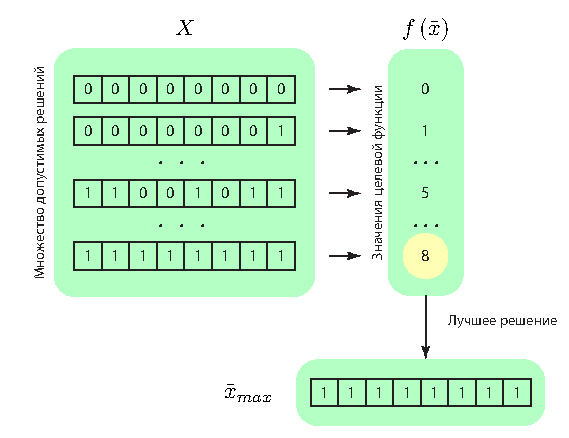
\includegraphics {ExampleProblemOptimization.pdf}
  \caption{Пример задачи оптимизации} 
  \label{StandardGA:img:ExampleProblemOptimization.pdf}  
\end{figure}


\clearpage